\documentclass[12pt, a4paper]{article}
\usepackage{geometry}
\usepackage{graphicx}
\usepackage{array}
\usepackage{lipsum}
\usepackage{boldline}

\usepackage[T2A,T1]{fontenc}

\usepackage[utf8]{inputenc}
\usepackage{times}
\usepackage[russian]{babel}
\renewcommand{\familydefault}{\sfdefault}

\begin{document}

\pagenumbering{gobble}

\newgeometry{noheadfoot=true,top=0.5cm,bottom=0.5cm, left=0.5cm, right=0.5cm}
\renewcommand{\arraystretch}{1.5}

\begin{figure}[t]
\scriptsize 
\begin{tabular}[b]{ V{2.8} m{2.0cm} V{2.8} m{6.2cm} V{2.8} m{2cm} V{2.8} m{5.85cm} V{2.8} } 
\hlineB{2.8}
Фамилия &  & Пол & \\  [0.45cm]
\hlineB{2.8}
Имя &  & Возраст & \\  [0.45cm]
\hlineB{2.8}

\end{tabular}

\includegraphics[scale=0.16]{imgs/marker_2171}
\end{figure}

\setlength{\textfloatsep}{5pt plus 1.0pt minus 1.0pt}

\begin{figure}[t]
\scriptsize 
\begin{tabular}[b]{ V{2.8} m{2.0cm} V{2.8} m{6.2cm} V{2.8} m{2.0cm} V{2.8}  m{8.0cm }V{2.8}} 
\hlineB{2.8}
Державинск &  & Кызылорда &  \\ [0.45cm]
\hlineB{2.8}
Ерейментау &  & Ленгер &  \\ [0.45cm]
\hlineB{2.8}
Есик &  & Лисаковск &  \\ [0.45cm]
\hlineB{2.8}
Есиль &  & Макинск &  \\ [0.45cm]
\hlineB{2.8}
Жанаозен &  & Мамлютка &  \\ [0.45cm]
\hlineB{2.8}
Жанатас &  & Павлодар &  \\ [0.45cm]
\hlineB{2.8}
Жаркент &  & Петропавловск &  \\ [0.45cm]
\hlineB{2.8}
Жезказган &  & Приозерск &  \\ [0.45cm]
\hlineB{2.8}
Жем &  & Риддер &  \\ [0.45cm]
\hlineB{2.8}
Жетысай &  & Рудный &  \\ [0.45cm]
\hlineB{2.8}
Житикара &  & Сарань &  \\ [0.45cm]
\hlineB{2.8}
Зайсан &  & Сарканд &  \\ [0.45cm]
\hlineB{2.8}
Зыряновск &  & Сарыагаш &  \\ [0.45cm]
\hlineB{2.8}
Казалинск &  & Сатпаев &  \\ [0.45cm]
\hlineB{2.8}
Кандыагаш &  & Семей &  \\ [0.45cm]
\hlineB{2.8}
Капчагай &  & Сергеевка &  \\ [0.45cm]
\hlineB{2.8}
Караганда &  & Серебрянск &  \\ [0.45cm]
\hlineB{2.8}
Каражал &  & Степногорск &  \\ [0.45cm]
\hlineB{2.8}
Каратау &  & Степняк &  \\ [0.45cm]
\hlineB{2.8}
Каркаралинск &  & Тайынша &  \\ [0.45cm]
\hlineB{2.8}
Каскелен &  & Талгар &  \\ [0.45cm]
\hlineB{2.8}
Кентау &  & Талдыкорган &  \\ [0.45cm]
\hlineB{2.8}
Кокшетау &  & Тараз &  \\ [0.45cm]
\hlineB{2.8}
Костанай &  & Текели &  \\ [0.45cm]
\hlineB{2.8}
Кульсары &  & Темир &  \\ [0.45cm]
\hlineB{2.8}
Курчатов &  & Темиртау &  \\ [0.45cm]
\hlineB{2.8}
\end{tabular}
\end{figure}

\newpage

\newgeometry{noheadfoot=true,top=0.5cm,bottom=0.5cm, left=0.5cm, right=0.5cm}
\renewcommand{\arraystretch}{1.5}

\begin{figure}[t]
\scriptsize 
\begin{tabular}[b]{ V{2.8} m{2.0cm} V{2.8} m{6.2cm} V{2.8} m{2cm} V{2.8} m{5.85cm} V{2.8} } 
\hlineB{2.8}
Фамилия &  & Пол & \\  [0.45cm]
\hlineB{2.8}
Имя &  & Возраст & \\  [0.45cm]
\hlineB{2.8}

\end{tabular}

\includegraphics[scale=0.16]{imgs/marker_2699}
\end{figure}

\setlength{\textfloatsep}{5pt plus 1.0pt minus 1.0pt}

\begin{figure}[t]
\scriptsize 
\begin{tabular}[b]{ V{2.8} m{2.0cm} V{2.8} m{6.2cm} V{2.8} m{2.0cm} V{2.8}  m{8.0cm }V{2.8}} 
\hlineB{2.8}
Туркестан &  & Бестобе &  \\ [0.45cm]
\hlineB{2.8}
Уральск &  & Ботакара &  \\ [0.45cm]
\hlineB{2.8}
Усть-Каменагорск &  & Горняцкий &  \\ [0.45cm]
\hlineB{2.8}
Ушарал &  & Гульшат &  \\ [0.45cm]
\hlineB{2.8}
Уштобе &  & Деркул &  \\ [0.45cm]
\hlineB{2.8}
Форт-Шефченко &  & Долинка &  \\ [0.45cm]
\hlineB{2.8}
Хромтау &  & Жайрем &  \\ [0.45cm]
\hlineB{2.8}
Шалкар &  & Жезказган &  \\ [0.45cm]
\hlineB{2.8}
Шар &  & Заводской &  \\ [0.45cm]
\hlineB{2.8}
Шардара &  & Затобольск &  \\ [0.45cm]
\hlineB{2.8}
Шахтинск &  & Зачаганск &  \\ [0.45cm]
\hlineB{2.8}
Шемонаиха &  & Индерборский &  \\ [0.45cm]
\hlineB{2.8}
Шу &  & Карабалык &  \\ [0.45cm]
\hlineB{2.8}
Шымкент &  & Качар &  \\ [0.45cm]
\hlineB{2.8}
Щучинск &  & Киевка &  \\ [0.45cm]
\hlineB{2.8}
Экибастуз &  & Конырат &  \\ [0.45cm]
\hlineB{2.8}
Эмба &  & Круглоозерное &  \\ [0.45cm]
\hlineB{2.8}
Новодолинский &  & Ленинский &  \\ [0.45cm]
\hlineB{2.8}
Айтеке би &  & Макат &  \\ [0.45cm]
\hlineB{2.8}
Аксу &  & Октябрьский &  \\ [0.45cm]
\hlineB{2.8}
Актас &  & Осакаровка &  \\ [0.45cm]
\hlineB{2.8}
Актау &  & Отеген батыра &  \\ [0.45cm]
\hlineB{2.8}
Аршалы &  & Сарыколь &  \\ [0.45cm]
\hlineB{2.8}
Атасу &  & Сарыозек &  \\ [0.45cm]
\hlineB{2.8}
Балпык &  & Саяк &  \\ [0.45cm]
\hlineB{2.8}
Белколь &  & Турлан &  \\ [0.45cm]
\hlineB{2.8}
\end{tabular}
\end{figure}

\newpage

\newgeometry{noheadfoot=true,top=0.5cm,bottom=0.5cm, left=0.5cm, right=0.5cm}
\renewcommand{\arraystretch}{1.5}

\begin{figure}[t]
\scriptsize 
\begin{tabular}[b]{ V{2.8} m{2.0cm} V{2.8} m{6.2cm} V{2.8} m{2cm} V{2.8} m{5.85cm} V{2.8} } 
\hlineB{2.8}
Фамилия &  & Пол & \\  [0.45cm]
\hlineB{2.8}
Имя &  & Возраст & \\  [0.45cm]
\hlineB{2.8}

\end{tabular}
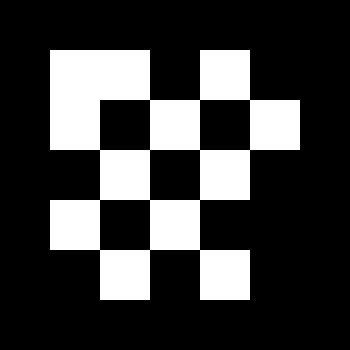
\includegraphics[scale=0.16]{imgs/marker_2773}
\end{figure}

\setlength{\textfloatsep}{5pt plus 1.0pt minus 1.0pt}

\begin{figure}[t]
\scriptsize 
\begin{tabular}[b]{ V{2.8} m{2.0cm} V{2.8} m{6.2cm} V{2.8} m{2.0cm} V{2.8}  m{8.0cm }V{2.8}} 
\hlineB{2.8}
Республика &  & Мангистауская &  \\ [0.45cm]
\hlineB{2.8}
Казахстан &  & Костанайская &  \\ [0.45cm]
\hlineB{2.8}
РК &  & Астана &  \\ [0.45cm]
\hlineB{2.8}
Область &  & Абай &  \\ [0.45cm]
\hlineB{2.8}
обл. &  & Акколь &  \\ [0.45cm]
\hlineB{2.8}
Город &  & Аксай &  \\ [0.45cm]
\hlineB{2.8}
г. &  & Аксу &  \\ [0.45cm]
\hlineB{2.8}
Район &  & Актау &  \\ [0.45cm]
\hlineB{2.8}
р-н &  & Актобе &  \\ [0.45cm]
\hlineB{2.8}
Село &  & Алга &  \\ [0.45cm]
\hlineB{2.8}
с. &  & Алматы &  \\ [0.45cm]
\hlineB{2.8}
Поселок &  & Аральск &  \\ [0.45cm]
\hlineB{2.8}
п. &  & Аркалык &  \\ [0.45cm]
\hlineB{2.8}
Атырауская &  & Арысь &  \\ [0.45cm]
\hlineB{2.8}
Алматинская &  & Атбасар &  \\ [0.45cm]
\hlineB{2.8}
Актюбинская &  & Атырау &  \\ [0.45cm]
\hlineB{2.8}
Акмолинская &  & Балхаш &  \\ [0.45cm]
\hlineB{2.8}
Жамбылская &  & Байконыр &  \\ [0.45cm]
\hlineB{2.8}
Аягоз &  & Булаево &  \\ [0.45cm]
\hlineB{2.8}
Восночно-Казахстанская &  & Бостандыкский  &  \\ [0.45cm]
\hlineB{2.8}
Западно-Казахстанская &  & Алмалинский &  \\ [0.45cm]
\hlineB{2.8}
Южно-Казахстанская &  & Медеуский &  \\ [0.45cm]
\hlineB{2.8}
Северо-Казахстанская &  & Каменка &  \\ [0.45cm]
\hlineB{2.8}
Карагандинская &  & Орбита &  \\ [0.45cm]
\hlineB{2.8}
Павлодарская &  & микрорайон &  \\ [0.45cm]
\hlineB{2.8}
Кызылординская &  & мкр. &  \\ [0.45cm]
\hlineB{2.8}
\end{tabular}
\end{figure}
\end{document}